\section{Zombieland II}
\subsection{Descripci\'on de la problem\'atica}

\textcolor{red}{Poner que la posicion final es bunker}

El escenario con el que vamos a trabajar es una ciudad tipo con \emph{n} calles horizontales y \emph{m} calles verticales. En esta ciudad se encuentran dispersos zombies, los mismos est\'an dispuestos en las calles (tanto en las verticales como en las horizontales) pero ninguno est\'a ubicado exactamente en alguna esquina. 

Contamos con \emph{s} soldados, los cuales se quieren movilizar desde una posici\'on inicial ($X_i$) hasta una posici\'on final ($X_f$).

Todos estos datos van a ser ingresados como par\'ametros de entrada.\\

Efectivamente, al encontrarse soldados con zombies se va a producir un enfrentamiento. Si la cantidad de soldados que se enfrentan con los zombies es mayor o igual, se exterminan los zombies de esa cuadra sin dejar ning\'un soldado muerto. 

En cambio, si la cantidad de zombies es mayor a la cantidad de soldados, se va a sufrir una baja de ($z-s$) soldados. De este modo, si $z-s\geq s$ toda la cuadrilla va a quedar eliminada impidiendo el avance con el recorrido. En caso contrario, se eliminan los zombies de esa cuadra perdiendo los $z-s$ soldados.

Esto implica el impedimento de recorrer un camino cuando $s=0$ (incluso cuando as\'i sea el par\'ametro de entrada) sin tener en cuenta la existencia o no de zombies en el trayecto restante.\\

Se busca hallar la manera de llegar desde $X_i$ hasta $X_f$ con la mayor cantidad de soldados sobrevivientes, si es posible. De haber m\'as de un camino que cumpla estas condiciones, se debe devolver s\'olo uno.\\

Se exige una cota de complejidad temporal de $\mathbf{O(s.n.m)}$.\\

\textcolor{red}{Insertar ejemplito con dibujo.}

\newpage
\subsection{Resoluci\'on propuesta y justificaci\'on}

Para modelar la problem\'atica planteada, utilizamos dos grafos.\\
\\

El \emph{primer grafo} (no dirigido) con el que vamos a tratar es el que almacena los datos de entrada -\texttt{ciudadInfestada}- (cantidad de zombies por cuadra), de modo que cada nodo es una esquina de la ciudad y cada eje tiene en su peso la cantidad de zombies que est\'an presentes en esa locaci\'on.\\
\\

El \emph{segundo grafo} (dirigido) -\texttt{grafo}- lo vamos a ir construyendo, de modo que al finalizarlo tengamos calculada la soluci\'on.\\

Cada nodo de \texttt{grafo} va a contener la siguiente informaci\'on: cantidad de soldados vivos con la que se lleg\'o a esa posici\'on (\texttt{soldadosVivos}) y las coordenadas de su posici\'on: \texttt{i} y \texttt{j}.

Los ejes de nuestro \texttt{grafo} no van a contener ninguna informaci\'on extra, s\'olo indicar\'an movimientos desde un nodo a otro que sean posibles. Es decir, s\'olo va a haber una conexi\'on del nodo \emph{e} al nodo \emph{f} si en ese trayecto no se produjo la baja total de los soldados.

\textcolor{red}{Poner un ejemplito que diga de un nodo e al f cuantos soldados se perdieron porque nos fijamos en ciudadInfestada}.\\



Lo primero que vamos a hacer es situarnos en la posici\'on inicial ($X_i = (inicioH, inicioV)$) y crear este nodo en \texttt{grafo}, de modo que \texttt{soldadosVivos} va a ser la cantidad de soldados inicial \textcolor{red}{... Llegue hasta aca, depsues continuo}


del grafo \texttt{ciudadInfestada}


\subsubsection*{PseudoC\'odigo}
\textcolor{red}{Poner un pseudo codigo del algoritmo.}
\subsection{An\'alisis de la complejidad}

\newpage

\subsection{C\'odigo fuente}
	\begin{codesnippet}
	\begin{verbatim}
    struct posYsold {
        int soldadosVivos;
        int i;
        int j;
    };
	\end{verbatim}
	\end{codesnippet}

	\begin{codesnippet}
	\begin{verbatim}
    Matriz ciudadInfestada;
    unsigned int n, m;
    
    int main(int argc, char const *argv[]){
        unsigned int s;
        cin >> n >> m >> s;
        unsigned int inicioH, inicioV, bunkerH, bunkerV;
        cin >> inicioH >> inicioV >> bunkerH >> bunkerV;
        inicioV--;
        inicioH--;
        bunkerV--;
        bunkerH--;
    //la matriz de la ciudad guarda cuantos zombies tiene el eje para moverse
    // a la derecha y hacia abajo (en ese orden)
    //para la izquierda es ir al de la izquierda y preguntar por el derecho
    //para arriba es ir al de arriba y preguntar por el de abajo
        ciudadInfestada = Matriz(n, vector<pair<int, int> >(m));
        for (int i = 0; i < n-1; ++i) {
            for (int j = 0; j < m-1; ++j) {
                cin >> ciudadInfestada[i][j].first;
            }
    //no hay camino a la derecha
            ciudadInfestada[i][m-1].first = -1;
            for (int j = 0; j < m; ++j) {
                cin >> ciudadInfestada[i][j].second;
            }
        }
        for (int j = 0; j < m-1; ++j) {
            cin >> ciudadInfestada[n-1][j].first;
    //no hay camino hacia abajo
            ciudadInfestada[n-1][j].second = -1;
        }
    //no hay camino a la derecha ni abajo
        ciudadInfestada[n-1][m-1].first = -1;
        ciudadInfestada[n-1][m-1].second = -1;
    //creamos el cubo a completar
        Cubo grafo(n, vector<vector<pair<posYsold, bool> > >(m));
        for (int i = 0; i < n; ++i) {
            for (int j = 0; j < m; ++j) {
                grafo[i][j] = vector<pair<posYsold, bool> >(s+1);
            }
        }
    //aplicamos el algoritmo
        int soldadosVivos = zombieland(grafo, inicioH, inicioV, bunkerH, bunkerV, s);
	\end{verbatim}
	\end{codesnippet}

	\begin{codesnippet}
	\begin{verbatim}
    //cout pedido
        cout << soldadosVivos << endl;
        deque<posYsold> recorrido;
    //para armarlo desde el principio hasta el final
        if(soldadosVivos != 0){
            posYsold posActual;
            posActual.soldadosVivos = soldadosVivos;
            posActual.i = bunkerH;
            posActual.j = bunkerV;
            while(posActual.i != inicioH || posActual.j != inicioV){
                recorrido.push_front(posActual);
                posActual = grafo[posActual.i][posActual.j][posActual.soldadosVivos].first;
            }
            posActual.soldadosVivos = s;
            posActual.i = inicioH;
            posActual.j = inicioV;
            recorrido.push_front(posActual);
        }
        for (int i = 0; i < recorrido.size(); ++i) {
            cout << recorrido[i].i+1 << " " << recorrido[i].j+1 << endl;
        }
        return 0;
    }
	\end{verbatim}
	\end{codesnippet}

	\begin{codesnippet}
	\begin{verbatim}
    int zombieland(Cubo& grafo, int inicioH, int inicioV, int bunkerH, int bunkerV, int soldados){
        int maxSoldados = 0;
    //cola para el BFS arranca con la posicion de donde salimos
        queue<posYsold> cola;
        posYsold actual;
        actual.soldadosVivos = soldados;
        actual.i = inicioH;
        actual.j = inicioV;
        cola.push(actual);
    //se marca esta posicion como visitada
        grafo[inicioH][inicioV][soldados].second = true;
        int zombies;
        int resultadoBatalla;
    //mientras tengamos algo para visitar (no sabemos si llegaremos al final)
        while(cola.size() > 0){
    //actual es el primero de la cola
            actual = cola.front();
        //si no estamos el final vemos si podemos ir a cada una de las cuatro direcciones
        //si es valido, no se mueren todos los soldados y no visite ese nodo, 
        //agregare el siguiente nodo a visitar
        //si ya lo visite, existe un camino que me lleva hasta ahi, 
        //ya fue encolado el camino que le sigue
            if(!(actual.i == bunkerH && actual.j == bunkerV)){
                zombies = zombiesCuadra(actual.i, actual.j, ARRIBA);
                resultadoBatalla = resulBatalla(actual.soldadosVivos, zombies);
                if(zombies != -1 && resultadoBatalla > 0 && !grafo[actual.i-1][actual.j]
                [resultadoBatalla].second){
                    posYsold arriba;
                    arriba.soldadosVivos = resultadoBatalla;
                    arriba.i = actual.i-1;
                    arriba.j = actual.j;
                    cola.push(arriba);
                    grafo[actual.i-1][actual.j][resultadoBatalla].second = true;
                    grafo[actual.i-1][actual.j][resultadoBatalla].first = actual;
                }
                zombies = zombiesCuadra(actual.i, actual.j, DER);
                resultadoBatalla = resulBatalla(actual.soldadosVivos, zombies);
                if(zombies != -1 && resultadoBatalla > 0 && !grafo[actual.i][actual.j+1]
                [resultadoBatalla].second){
                    posYsold der;
                    der.soldadosVivos = resultadoBatalla;
                    der.i = actual.i;
                    der.j = actual.j+1;
                    cola.push(der);
                    grafo[actual.i][actual.j+1][resultadoBatalla].second = true;
                    grafo[actual.i][actual.j+1][resultadoBatalla].first = actual;
                }
	\end{verbatim}
	\end{codesnippet}

	\begin{codesnippet}
	\begin{verbatim}
                zombies = zombiesCuadra(actual.i, actual.j, ABAJO);
                resultadoBatalla = resulBatalla(actual.soldadosVivos, zombies);
                if(zombies != -1 && resultadoBatalla > 0 && !grafo[actual.i+1][actual.j]
                [resultadoBatalla].second){
                    posYsold abajo;
                    abajo.soldadosVivos = resultadoBatalla;
                    abajo.i = actual.i+1;
                    abajo.j = actual.j;
                    cola.push(abajo);
                    grafo[actual.i+1][actual.j][resultadoBatalla].second = true;
                    grafo[actual.i+1][actual.j][resultadoBatalla].first = actual;
                }
                zombies = zombiesCuadra(actual.i, actual.j, IZQ);
                resultadoBatalla = resulBatalla(actual.soldadosVivos, zombies);
                if(zombies != -1 && resultadoBatalla > 0 && !grafo[actual.i][actual.j-1]
                [resultadoBatalla].second){
                    posYsold izq;
                    izq.soldadosVivos = resultadoBatalla;
                    izq.i = actual.i;
                    izq.j = actual.j-1;
                    cola.push(izq);
                    grafo[actual.i][actual.j-1][resultadoBatalla].second = true;
                    grafo[actual.i][actual.j-1][resultadoBatalla].first = actual;
                }
            }
        //si llegamos al final, actualizamos los soldados que quedaron vivos, 
        //si es mayor a haber llegado por otro camino
            else
                if(maxSoldados < actual.soldadosVivos)
                    maxSoldados = actual.soldadosVivos;
        //desencolo el nodo que estaba analizando
            cola.pop();
        }
        return maxSoldados;
    }
	\end{verbatim}
	\end{codesnippet}

	\begin{codesnippet}
	\begin{verbatim}
    int zombiesCuadra(int i, int j, movimiento mov){
    //devuelve los zombies que en la cuadra pedida
        switch(mov){
            case ARRIBA:
                if(i == 0)
                    return -1;
                return ciudadInfestada[i-1][j].second;
            case ABAJO:
                return ciudadInfestada[i][j].second;
            case IZQ:
                if(j == 0)
                    return -1;
                return ciudadInfestada[i][j-1].first;
            case DER:
                return ciudadInfestada[i][j].first;
        }
    }
	\end{verbatim}
	\end{codesnippet}

	\begin{codesnippet}
	\begin{verbatim}
    int resulBatalla(int sold, int zomb){
    //devuelve si es posible pasar por una cuadra
        if(sold>=zomb)
            return sold;
        return sold-(zomb-sold); 
    }
	\end{verbatim}
	\end{codesnippet}

\newpage

\subsection{Experimentaci\'on}
\subsubsection{Constrastaci\'on Emp\'irica de la complejidad}

Al momento de llevar a cabo la experimentaci\'on, se consideró como\emph{ peor caso}, aquel en el que se debiera recorrer cada nodo de la ciudad (\texttt{grafo}), tantas veces como cantidad de soldados se tuviese a disposici\'on en el momento inicial. Es decir, pasar por cada esquina de la ciudad $s$ veces, cada vez con una cantidad diferente de \texttt{soldadosVivos}. Siendo ese caso, en el que se recorren $s.n.m$ elementos, coiniciendo así con la complejidad teórica $\mathbf{O(s.n.m)}$.\\

Aunque este ser\'ia el caso deseable, generar dicha instancia para los distintos valores de $s$, $n$ y $m$, resultó tan dificultoso como resolver el problema en cuestión. Por este motivo, se decidi\'o generar instancias con una cantidad aleatoria de zombies por cuadra.
Primero analizaremos con detalle estas instancias, y luego expondremos porque decidimos usarlas.

Al proceder bajo este m\'etodo fue posible efectuar casos de prueba de gran tamaño. Sin embargo, debido a la dimensi\'on de los casos de tests, hay ciertos aspectos de la soluci\'on del problema que no podemos determinar por nuestra cuenta para contrastar con la soluci\'on propuesta por el algoritmo:

\begin{enumerate}
	\item No se puede determinar si existe un camino desde el punto de inicio ($X_i$) hasta el búnker ($X_f$).
	\item No se puede determinar, si al existir un camino, este será único. 
	\item No se puede determinar cu\'antos soldados van a llegar al búnker.
	\item No se puede determinar cu\'antos caminos adulteran la cantidad de soldados, ni cu\'antos soldados mueren en cada uno de ellos.
\end{enumerate}

\textcolor{green}{TODO LA EXPLICACION ESTA, ESTA ABAJO: De este modo, al ejecutar nuestro algoritmo bajo las instancias aleatorias generadas, obtenemos soluciones para las cuales no podemos contrastar con otros valores para mostrar su correctitud. }\\

\textcolor{red}{Aca poner algo del estilo ``Como queremos probar instancias que se acerquen lo mejor posible al peor caso, generamos instancias probabilisticas que agranden lo mejor posible la complejidad''}
\textcolor{green}{Esto queda explicado en el parrafo anterior}\\

\textcolor{red}{Aca poner qu\'e es el generador de instancias, que es un laberitno y que represneta antes de mandar el dibujo :)}
\textcolor{green}{Abajo esta la explicacion del laberinto. En cuanto al generador de instancias... Es lo que explique abajo tambien (el laberinto muestra lo que devuelve el generador, y yo explique como arma el casos, o sea, eso de que devuelve entre 0 y s+1, o 0 y s*2, etc}
El resultado del generador de instancias, proporcionaba un laberinto como el siguiente:

\begin{center}
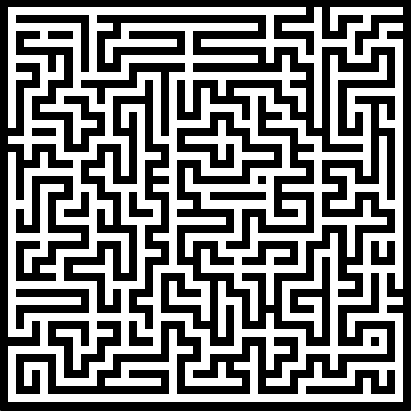
\includegraphics[width=7cm,keepaspectratio=yes]{imagenes/ej2/maze.png}
\end{center}

\textcolor{red}{Desde aca...}
Los pasajes del laberinto son los caminos donde hay entre $0$ y $s+1$ zombies, y las paredes, caminos donde hay entre $0$ y $s$.2.

Vale aclarar, que las paredes no necesariamente constituyen un medio por el cual los soldados no puedan pasar, sino un medio donde lograrlo es poco probable. Los pasajes, de modo similar, no necesariamente constituyen un medio por el cual los soldados siempre pueden pasar, sino un medio donde tener bajas, es poco probable.

Estos valores aleatorios fueron tomados adrede, por un lado, para que incluso el mejor camino (alguno de los pasajes que conducen a la salida), tuviera perdida de soldados, pero intentando que éstas sean mínimas, para aumentar las probabilidades de que puedan efectivamente llegar al búnker.\\

Aún asi, el $s$ tomado en el algoritmo aleatorio es el que se recibe en la entrada. Esto significa, que se configura al principio, y despues no se actualiza con la cantidad de soldados despues de una batalla.

Por ende, no podemos determinar el porcentaje de soldados totales que llegarán, pero sí podemos saber el porcentaje que sobrevivirá a la primer batalla, en el peor de los casos.

Así, la cantidad de soldados que sobreviviran a la primer batalla, en el peor caso, es:
\begin{itemize}
	\item Si toma un pasaje, en el peor de los casos, sobrevivirá el 50\% de los soldados (casos en el que hay 1 soldado y 2 zombies). No obstante, ese porcentaje tiende a 100\% a medida que la cantidad de soldados aumenta.
	\item Si toma una pared, solo sobrevivirá un 50\%, sin importar la cantidad de soldados.
\end{itemize}
\textcolor{red}{que es pasaje o pared?}\\
\textcolor{green}{Ahi arriba intente explicar un poco, te gusta mas?}

Estos rangos aleatorios se obtuvieron experimentando con distintas distribuciones de zombies, hasta lograr valores que ocasionaran bajas pero que no impidieran a los soldados llegar al búnker en la mayoría de los casos. Dichos experimentos exceden el interés de esta sección y no serán discutidos.\\

\bigskip

\textcolor{green}{Aca es donde explico porque decidimos usar estas instancias aunque no sean peor caso}
Finalmente, y pese a las dificultades expuestas, se decidió proceder con dichas instancias, tomandose solo aquellas donde se pudo asegurar que existía un camino al búnker, y que existía un camino donde hubiera al menos una baja (no necesariamente, estos dos sean el mismo camino), ya que lograban generar una fluctuación en la cantidad de soldados, y esto, si bien lejos del peor caso propuesto, resultó ser una aproximación que consideramos suficiente.
Para obtenerlas, se generaron instancias hasta obtener una que tuviera dichas características.\\

Consecuentemente, se realizaron experimentos sobre los siguientes dos casos:
\begin{itemize}
	\item \textbf{Cero zombies}: En esta instancia, la cantidad de zombies en cada cuadra es cero, con lo cual, el algoritmo recorre toda la ciudad, y se queda con cualquier camino.
	\item \textbf{Zombies aleatorios}: Es la instancia explicada anteriormente.
\end{itemize}

También es necesario aclarar, que los experimentos se realizaron sobre ciudades cuadradas, con puntos de inicio y llegada en los extremos opuestos de la ciudad, y con cantidad de soldados iniciales igual a 20. 
Tomamos esta decision porque los casos de ciudades cuadradas y de ciudades rectangulares, son análogos, dado que lo importante es la cantidad de cuadras en total. En lo que respecta a los puntos de partida y llegada, fueron elegidos para aprovechar al maximo la dimension de la ciudad y obtener el más largo de los caminos posibles.\\

A continuación se detallan los experimentos y sus resultados.
Debido al tamaño de las instancias de prueba, los inputs de dichos experimentos no fueron adjuntados.
\begin{center}
	\begin{tabular}{|c|c|c|}
	\hline
	Experimento & \textbf{Cero zombies} & \textbf{Zombies aleatorios}\\
	\hline
	\hline
	Tamaño de la ciudad & \multicolumn{2}{|c|}{Soldados al final}\\
	\hline
	50x50 & 20 & 6\\
	\hline
	100x100 & 20 & 19\\
	\hline
	250x250 & 20 & 17\\
	\hline
	500x500 & 20 & 17\\
	\hline
	750x750 & 20 & 16\\
	\hline
	1000x1000 & 20 & 12\\
	\hline
	1250x1250 & 20 & 20\\
	\hline
	1500x1500 & 20 & 7\\
	\hline
	1750x1750 & 20 & 14\\
	\hline
	2000x2000 & 20 & 20\\
	\hline
	\end{tabular}
\end{center}



\newpage

\subsubsection*{Cero Zombies}

Dado que los tiempos de ejecución para ambos experimentos varían ampliamente, primero analizaremos el experimento de \textbf{Cero zombies}.

\includegraphics[width=15cm,keepaspectratio=yes]{imagenes/ej2/czneto.png}

Como se puede apreciar, al no haber zombies, no existe ningun camino en el cual mueran soldados, por lo que los tiempos se incrementan acorde a la dimension de la ciudad, y al ser cuadradas, posee un crecimiento cuadrático. Más adelante justificaremos por qué pensamos que el gráfico es una función cuadrática y no de un grado mayor.

\newpage

\subsubsection*{Cero Zombies vs Zombies Aleatorios}

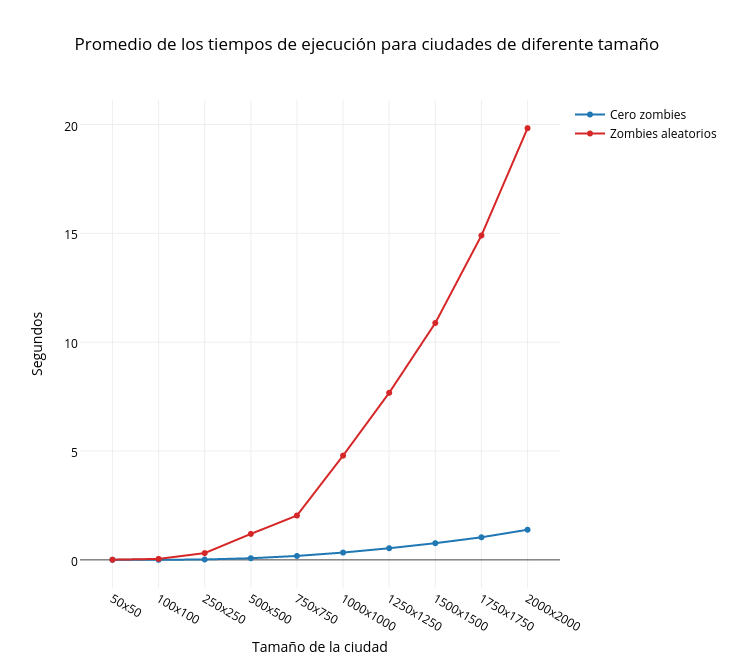
\includegraphics[width=15cm,keepaspectratio=yes]{imagenes/ej2/czyza.png}

Aquí se pueden apreciar las diferencias de tiempos. Ésta radica en el hecho de que \textbf{Zombies aleatorios} posee caminos en los cuales los soldados mueren. Por ello, el algoritmo deberá recorrer, en peor caso, $s$ veces la ciudad entera. En cambio, en el caso de \textbf{Cero Zombies} s\'olo arma una ``capa'' de la ciudad, es decir todos los nodos para las esquinas de la ciudad pero siempre \texttt{soldadosVivos}$=0$. \\

\newpage
Se procedió, entonces, a dividir los resultados de \textbf{Zombies aleatorios} por la cantidad de soldados iniciales con los que se ejecutó el algoritmo a fin de que quede reflejado, que en ese caso, los tiempos serán muy similares a los de \textbf{Cero zombies}. Esto se debe a que ya no son los tiempos de recorrer $s$ veces la ciudad, sino de recorrerla una sola vez y por ende, debe ser una función cuadrática.

Sin embargo, es necesario aclarar que la similitud que se intenta mostrar, es aproximada, ya que no podemos asegurar que efectivamente, el algoritmo recorre $s$ veces la ciudad. Tal es el peor caso, y como hemos expuesto en un principio, no podemos asegurar que sea el que realmente ocurre.

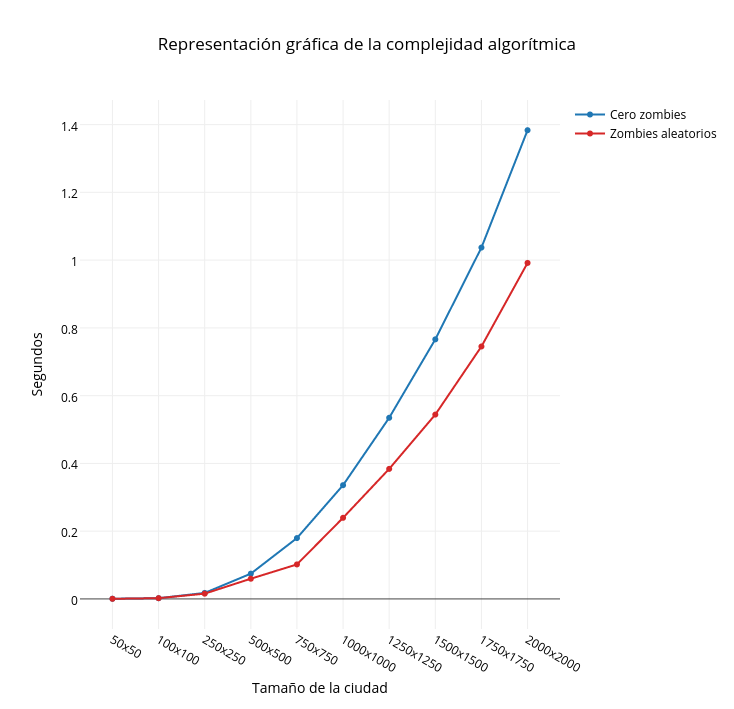
\includegraphics[width=15cm,keepaspectratio=yes]{imagenes/ej2/zaczados.png}

Tal como era esperado, en este grafico se muestran dos funciones cuadráticas, que como se explico anteriormente, solo difieren en la constante que las multiplica.

\newpage

Manteniendo los resultados de \textbf{Zombies aleatorios} divididos por $s$, finalmente dividimos los resultados tanto de \textbf{Cero zombies} como de \textbf{Zombies aleatorios}, por $n$, y en una instancia aparte, por $n.m$.

De esta manera, dado que en ambos tienen $s$ igual a 1, solo queda ver que al dividir por $n$, los resultados se aproximan a una función lineal, y que al dividirlos por $n.m$, se aproximan a una constante.\\

Como s\'olo nos interesa la relación, y no la función exacta ni la constante, multiplicamos los resultados de dichas divisiones por 100, para que los valores sean más claros y visibles.\\
\\

El gr\'afico siguiente corresponde a los tiempos de ejecuci\'on divididos por $s.n$ en el caso de \textbf{Zombies aleatorios}  y por $n$ en el caso de \textbf{Cero zombies}.

\includegraphics[width=15cm,keepaspectratio=yes]{imagenes/ej2/linealizacion.png}

Como se puede apreciar, el gráfico ahora muestra una función lineal, con lo cuál se inclina a demostrar que en el primer gráfico, la función representada era una función cuadrática.
Sin embargo, volveremos a realizar la división para asegurarnos que ésta función, es realmente una función lineal.

\newpage

El gr\'afico siguiente corresponde a los tiempos de ejecuci\'on divididos por $s.n.m$ en el caso de \textbf{Zombies aleatorios}  y por $n.m$ en el caso de \textbf{Cero zombies}.

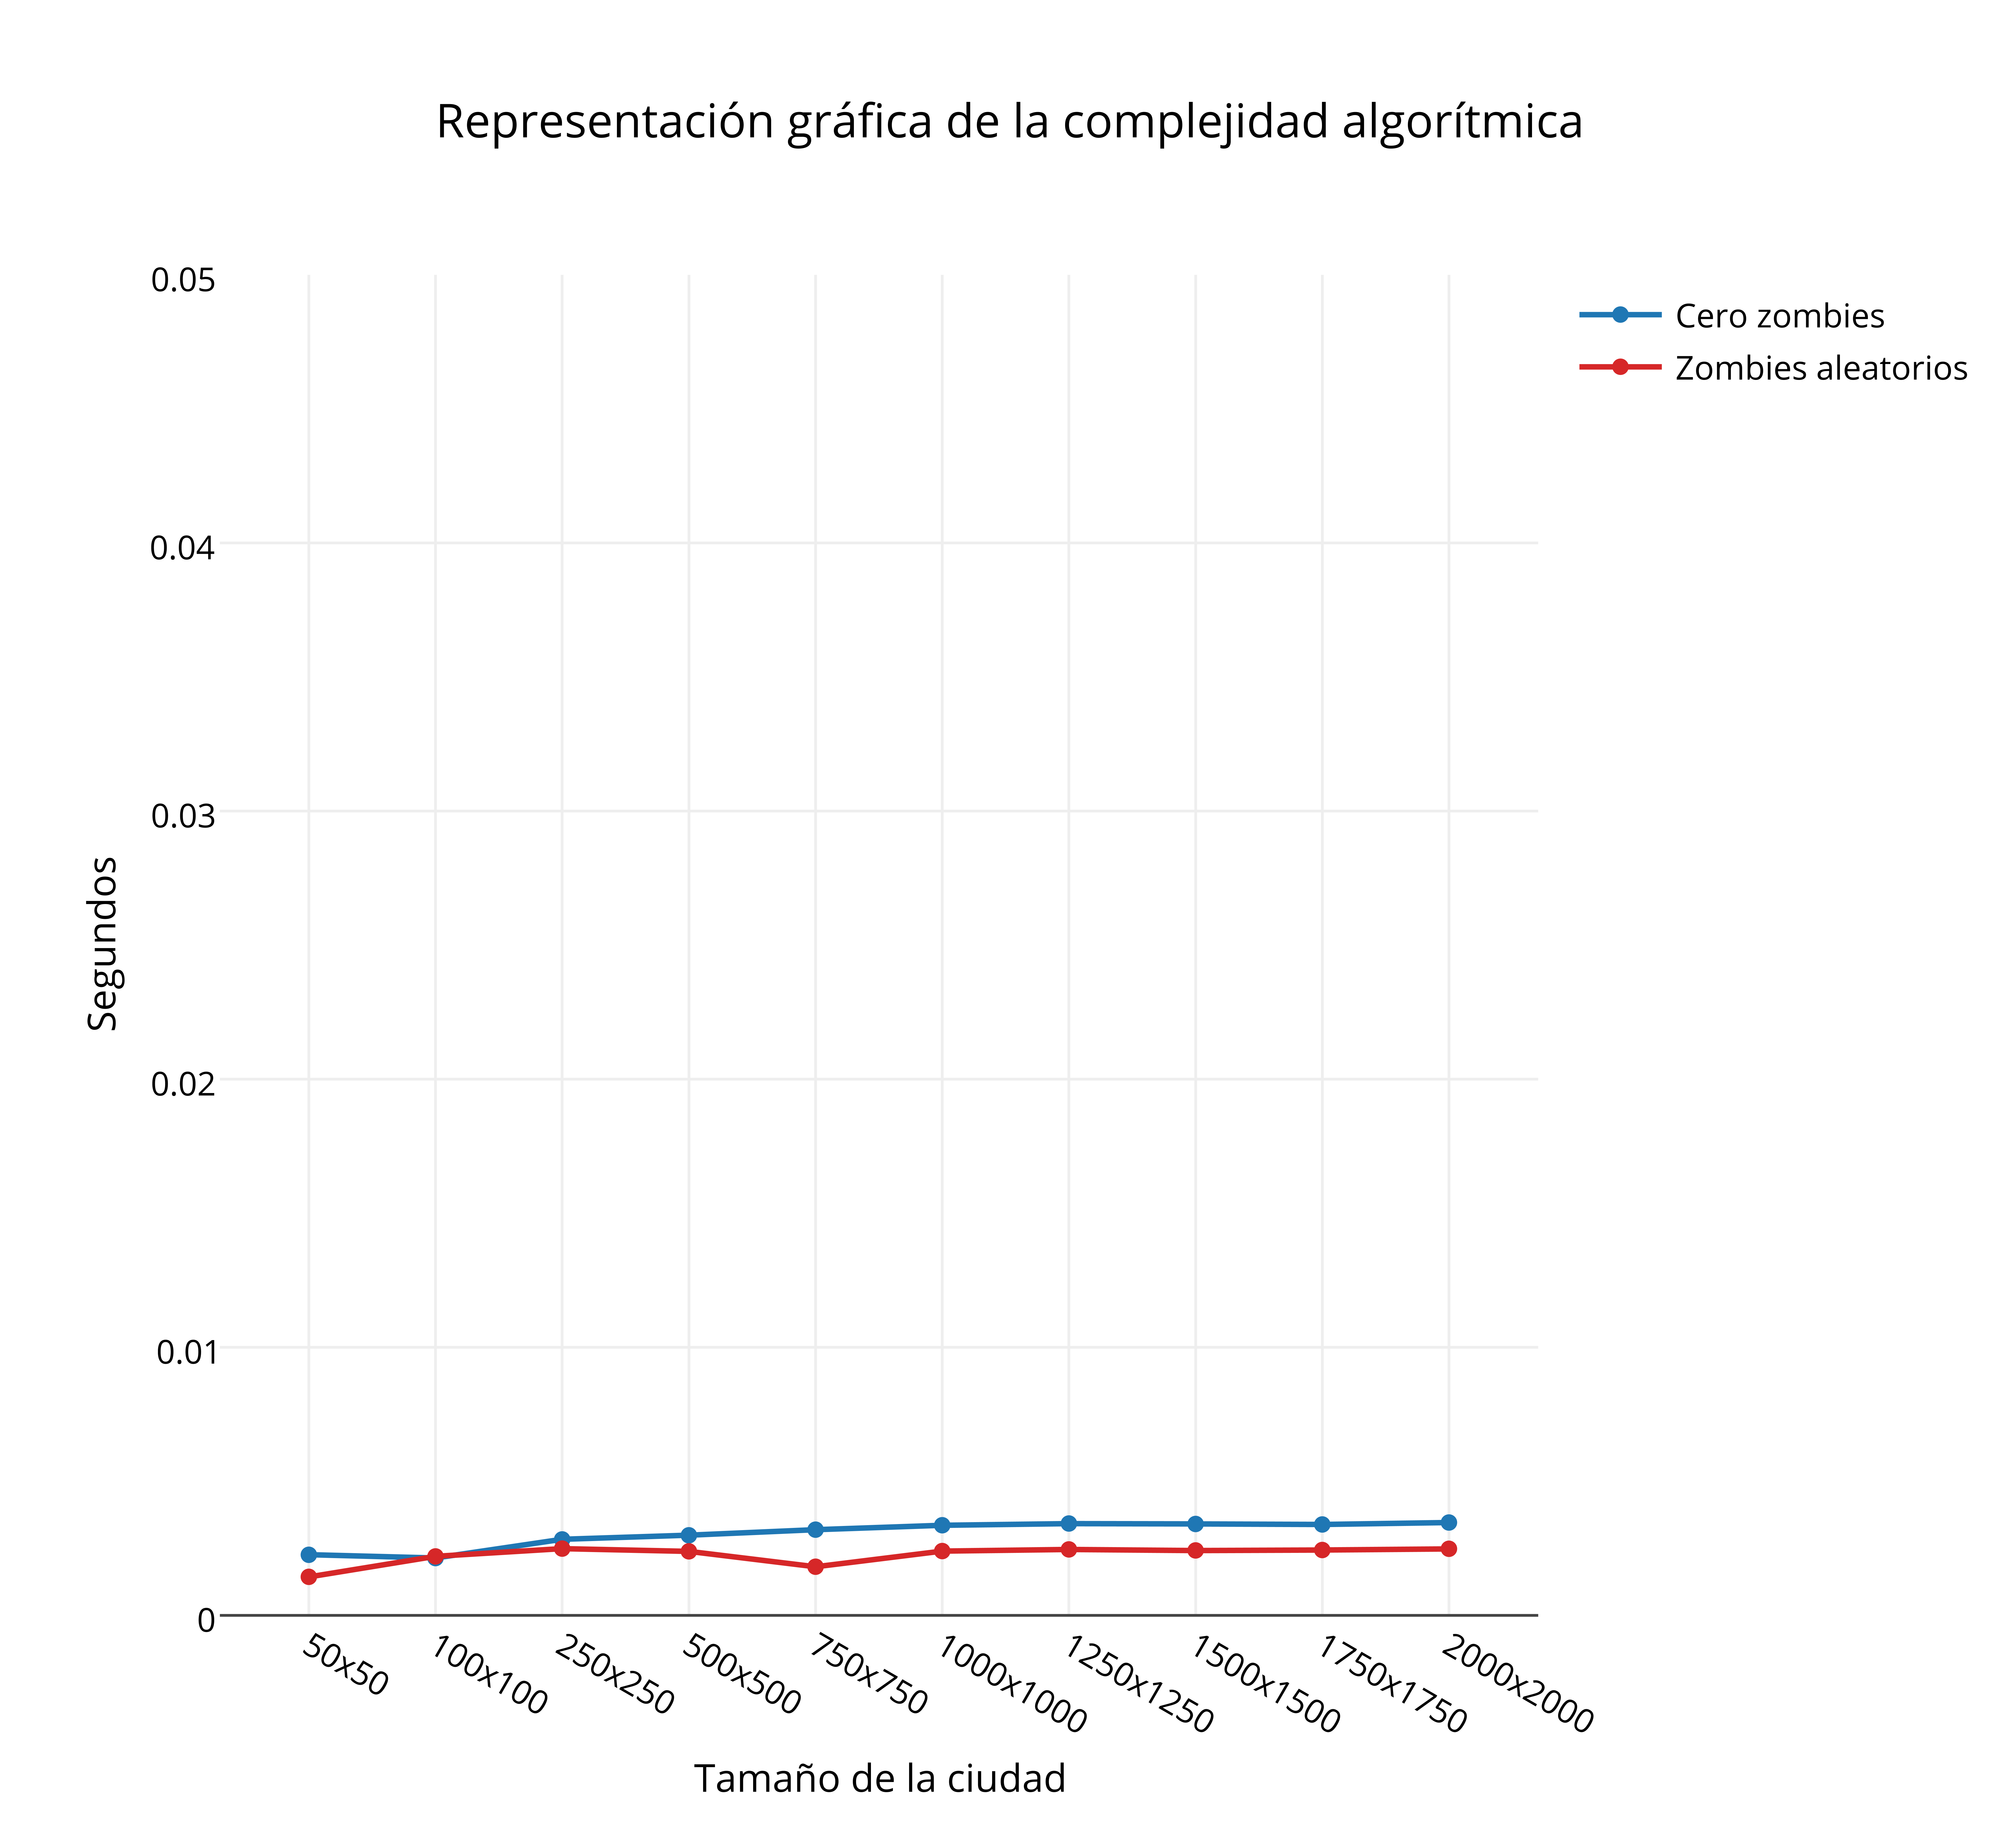
\includegraphics[width=15cm,keepaspectratio=yes]{imagenes/ej2/constantizacion.png}\

Efectivamente, el resultado de la división es una constante, y con esto se muestra que la primer función graficada, correspondía a una función cuadrática.

\bigskip

Se puede ver que la experimentación se corresponde con la teoría, y que la complejidad, en peor caso, es $\mathbf{O(s.n.m)}$.

